\chapter[Estratégias evolutivas para o PRM]{Estratégias evolutivas para o PRM}

A modelagem de um algoritmo genético para o problema do roteamento multicast não é trivial, pois a solução não pode ser representada por um vetor. De fato, como deve representar os caminho entre o servidor e os múltiplos destinos em uma rede de computadores, a solução para o PRM é uma árvore. Dessa forma, é preciso desenvolver o processo de crossover e de mutação de acordo com a estrutura. O cruzamento deve receber duas árvores e gerar uma nova que compartilha características de ambos os pais, enquanto a mutação precisa criar uma pequena alteração na árvore que permita melhor explorar o espaço de busca, mas que não a descaracterize completamente.

Em contrapartida, o PRM se aproxima da definição original do ACO, pois trabalha com grafos. A diferença está no fato de que a solução é representada por uma árvore ao invés de um simples caminho, fazendo com que o depósito de feromônio e a escolha de arestas sejam desenvolvidas conforme a nova estrutura.

\section{Representação da solução}

Como mostrado na seção [seção do prm], considerando que em cada nó da rede a mensagem pode ser replicada e enviada aos próximos nós conectados, o PRM deseja encontrar a árvore que representa o processo de transmissão de menor custo que parte do nó fonte (servidor) e atinge todos os destinos. Existem duas maneiras de se representar a solução:

\begin{enumerate}
	\item Representação em árvore: o AG evolui a própria árvore que se deseja encontrar como solução. É um processo mais complicado que a alternativa a seguir, mas nenhum pós-processamento é necessário.
	\item Representação em conjunto: o AG evolui um conjunto de caminhos $C$, ou seja, para cada nó destino $d$ no problema deve existir uma lista de nós $L \in C$ que contém a sequência de nós, onde o primeiro elemento é o servidor e o último é $d$. A representação em conjuntos é mais fácil de se gerenciar, mas exige a transformação em árvore ao final do processo. Como diferentes árvores podem ser formadas a partir de um conjunto de caminhos, essa representação não é tão eficiente quanto a anterior ao explorar o espaço de busca.
\end{enumerate}

Neste trabalho optou-se por utilizar a representação 1, árvores.

\section{Inicialização dos indivíduos}

\section{Cruzamento (AG)}

O modelo de cruzamento para o PRM utilizado neste trabalho é chamado de cruzamento por caminho e foi proposto em [dissertacao do Fialho] como uma alternativa ao cruzamento por similaridade utilizado em trabalhos anteriores [Bueno e Oliveira, 2010].

O cruzamento por caminho é realizado entre duas árvores $P_1$ e $P_2$ e produz um único filho $F$. O processo consiste em separar cada um dos pais em ramos e então, para cada nó destino $d$ do PRM, acrescentar a $F$ ou o ramo de $P_1$ que leva a $d$, ou o ramo de $P_2$. A escolha entre $P_1$ e $P_2$ é feita de forma aleatória. Assim que todos os nós destinos são atingíveis em $F$, para-se a seleção de ramos, remove-se os ciclos que possivelmente foram incluídos e poda-se a árvore, excluindo qualquer nó folha que não seja um destino.

\begin{figure}[!htbp]
	\label{fig_prm-cruzamento-caminho}
	\caption{Exemplo de cruzamento por caminho}
	\centering
	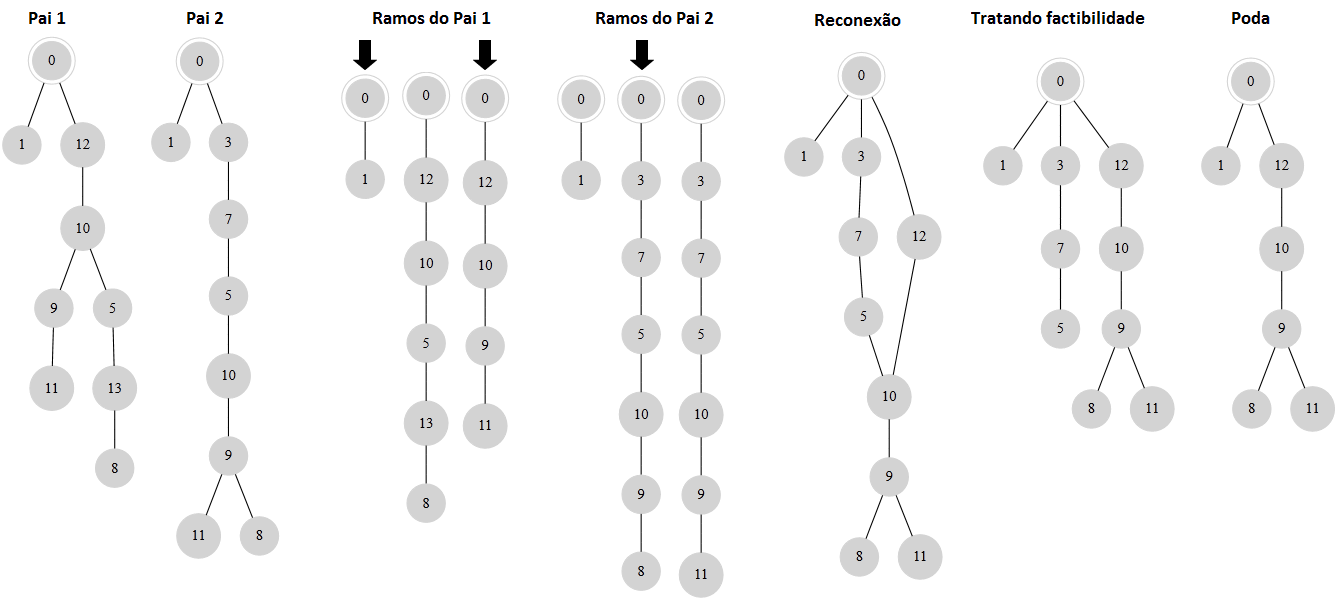
\includegraphics[width=1\textwidth]{cap_estrategias-prm/figs/prm-cruzamento-caminho}
\end{figure}

A figura \ref{fig_prm-cruzamento-caminho}, retirada do trabalho de [dissertacao Fialho], representa o processo de cruzamento por caminho entre duas árvores (Pai 1 e Pai 2). No exemplo, o nó raiz (servidor) é o vértice 0 e os destinos são o conjunto $\{1, 8, 11\}$. As setas em ``ramos do pai 1'' e ``ramos do pai 2'' representam os caminhos escolhidos em cada um dos pais para compor a árvore filha. O grafo nomeado ``reconexão'' representa o filho após a inclusão de todos os ramos, e como foi gerado um ciclo, deve-se removê-lo afim de obter-se uma árvore válida. Em ``tratando factibilidade'' apresenta-se o filho após a remoção dos ciclos, como o nó folha ``5'' não é um destino, deve-se podá-lo, resultando na última árvore, ``poda'', que é o filho retornado pelo processo.

Durante o processo de cruzamento por caminho, para remover os ciclos, percorre-se a árvore em largura removendo qualquer aresta que adicione ciclo. No processo de poda, verifica-se todas as folhas, se alguma não for um destino, remove-se o nó, repetindo o processo até que todos os nós folhas sejam destinos.

\section{Mutação (AG)}

A mutação em uma árvore que representa uma solução para o PRM consiste em remover parte dos nós da árvore e então reconectá-los de maneira aleatória utilizando o grafo correspondente à rede em questão. Veja o algoritmo \ref{alg_prm_mutacao}.

\begin{algorithm}
	\caption{Mutação para uma árvore $(A, G, qte_{arestas}, r, D)$}
	\label{alg_prm_mutacao}
	\begin{algorithmic}[1]
		\State Selecione aleatoriamente $qte_{arestas}$ e remova-as de $A$
		\State Retire de $A$ a componente conexa que contém a raiz e chame-a de $C$
		\State Crie um grafo vazio $M$ para guardar o resultado da mutação
		\State Adicione todas as arestas de $C$ a $M$
		\While{$|D| > 0$}
			\State Selecione aleatoriamente um destino $d \in D$ e remova-o da lista $D$
			\State Remova de $A$ a componente conexa correspondente ao destino $d$ e coloque-a em $C$
			\If{$M$ não possui o vértice $d$}
				\State Tendo $G$ como referência, crie um caminho aleatório $P$ entre $M$ e a componente conexa $C$
				\State Adicione todas as arestas de $P$ a $M$
			\EndIf
			\State Adicione todas as arestas de $C$ a $M$
		\EndWhile
		\State Remova os ciclos em $M$, caso existam
		\State Pode a árvore $M$, removendo todos os nós folhas que não são destinos
		\State \Return $M$
	\end{algorithmic}
\end{algorithm}

No algoritmo \ref{alg_prm_mutacao} recebe-se como parâmetros a árvore a se mutar ($A$), o grafo da rede ($G$), a quantidade de arestas a se remover na mutação ($qte_{arestas}$), o vértice raiz ($r$), e o conjunto de destinos ($D$). Na linha 7, se não existe componente conexa com o vértice $d$, $C$ será um grafo com um único nó ($d$) e nenhuma aresta. Na linha 9, o caminho aleatório é construído nó a nó até se encontrar uma sequência de arestas entre as duas componentes. Ao final, o mesmo pós-processamento do cruzamento por caminho é realizado: remove-se os ciclos e poda-se a árvore.

\section{Construção da solução (ACO)}

O processo de construção da solução por um ACO no PRM deve gerar a árvore multicast com base no grafo da rede, da estrutura de feromônios e da heurística. Existem diversas maneiras de se criar tal árvore. A fim de estudar o comportamento das diferentes estratégias possíveis, aprimorá-las e determinar o melhor modelo para se utilizar no PRM, analisou-se o comportamento de cada ideia no caso mais básico possível: o PRM mono-objetivo. As ideias consideradas neste trabalho são listadas a seguir:

\begin{enumerate}
	\item A primeira estratégia, apresentada em [Baran PRM], pode ser vista como uma formiga que caminha pelo grafo até encontrar todos os destinos. A análise é feita passo a passo, considerando apenas a vizinhança do vértice corrente como possibilidades para compor a solução. O processo inicia com uma lista de exploração ($E$) que contém um único elemento: a raiz. Sorteia-se um vértice $i \in E$ e atribui-se probabilidades a todas as arestas $(i, j)$, onde $j$ é qualquer vértice não-visitado na vizinhança de $i$. $i$ é removido de $E$ caso não possua vizinhos factíveis. Um vértice $v$ é escolhido de acordo com as probabilidades calculadas, a aresta $(i, v)$ é adicionada à solução e $v$ é inserido na lista de exploração $E$. O processo é repetido até que todos os destinos tenham sido alcançados. Como etapa final, poda-se a árvore, eliminando as folhas que não representam destinos.
	\item A solução pode ser vista como os caminhos entre a raiz e cada um dos destinos, portanto, outra estratégia é imaginar que $|D|$ formigas partirão da raiz e cada uma deve encontrar um vértice $d \in D$ diferente, onde $D$ é o conjunto de nós destinos. Com cada um dos caminhos em mãos, monta-se a árvore com o cuidado de não se incluir ciclos. O último passo é a poda, que exclui qualquer vértice folha que não seja um destino. %mants
	\item Uma terceira estratégia, proposta neste trabalho, representa uma formiga fictícia que pode estar em vários locais do grafo ao mesmo tempo. Dessa forma, é possível analisar as probabilidades de todas as arestas factíveis ao mesmo tempo, ao invés de sempre escolher a composição da solução de acordo com uma vizinhança local. Ao considerar todas as possibilidades ao mesmo tempo, obtém-se um processo melhor de decisão que não tende o resultado para algum dos ramos da árvore, já que a todo momento, qualquer vértice factível pode ser incluído no resultado. O processo é iniciado a partir de uma lista de exploração ($E$) que contém todas as arestas com uma extremidade na raiz. A cada passo, calcula-se as probabilidades para toda aresta de $E$ e, de acordo com os valores obtidos, escolhe-se $e \in E$ para compor a solução. $e$ é então removido de $E$, adicionado à solução e tem todas as arestas com que compartilha um vértice adicionadas à lista de exploração (desde que ainda não tenham sido incluídas). O processo é repetido até que todos os destinos sejam atingidos. Uma poda é realizada ao final do algoritmo.
	\item Uma última estratégia é fazer um processo inverso para se construir a solução, ao invés de partir da raiz e chegar nos destinos, este modelo propõe que se utilize $|D|$ formigas, onde cada uma tem como posição inicial um destino $d \in D$ diferente. $D$ é o conjunto de vértices destinos. A ideia é que as formigas escolham seus caminhos localmente com base nas probabilidades das arestas em suas vizinhanças. Sempre que uma formiga encontrar o caminho que já foi explorado por outra formiga, ela para de explorar e meio e segue os mesmos passos realizados pelo outro agente. O processo termina quando o nó raiz foi encontrado por alguma formiga e todas as formigas tiverem se encontrado. Em linguagem matemática, o processo inicia com uma componente conexa para cada $d \in D$. Em todo passo do algoritmo, cada componente conexa é explorada a partir do último nó adicionado. Em cada componente, calcula-se as probabilidades das arestas na vizinhança do nó sendo explorado e escolhe-se, de acordo com os valores obtidos, uma novo vértice $v$ para ser adicionado à componente. Se não há arestas factíveis na vizinhança, deve-se rebobinar a exploração para um vértice anterior. Caso o nó incluído $v$ pertença a uma outra componente conexa, une-se as duas estruturas. O processo termina quando existe apenas uma componente conexa e o vértice raiz foi encontrado. Uma poda é realizada como pós-processamento da árvore. 
\end{enumerate}

Cada uma das estratégias mencionadas foi implementada e testada a fim de determinar aquela que produz as soluções de melhor qualidade. O PRM com apenas um objetivo foi o problema escolhido para avaliá-las. A fim de obter um valor como parâmetro de qualidade, também foi implementada uma versão modificada do algoritmo de Prim que aproxima a árvore multicast de menor custo. Como esperado, o algoritmo de Prim é uma opção melhor que o ACO quando se trata do PRM mono-objetivo, mas a intenção deste estudo não foi produzir um algoritmo melhor para o problema, mas sim testar as estratégias de construção de solução com o fim de utilizá-las em versões mais complexas (multi-objetivas) do PRM.

Os resultados do testes, que podem ser encontrados no apêndice [], mostraram que a estratégia número 3 representa a melhor relação entre qualidade do resultado e tempo de execução. Portanto, para todos os experimentos no PRM da seção [], esse foi o método de construção da solução utilizado.

Na lista acima, a estratégia número 3, escolhida como a melhor forma de se construir uma solução para o PRM no ACO, é explicada de maneira geral e omite alguns detalhes que são expressos no algoritmo \ref{alg_aco_prm_construir_solucao}. A ideia principal se mantem a mesma, mas se implementada da maneira como foi escrita, se torna um processo muito lento. É possível agilizar o algoritmo, sem afetar muito a qualidade das soluções, através de algumas técnicas de amostragem.

\begin{algorithm}
	\caption{Geração de solução no ACO $(G, r, D, \tau, h, E'_{size})$}
	\label{alg_aco_prm_construir_solucao}
	\begin{algorithmic}[1]
		\State Inicie uma árvore vazia $T$
		\State Inicie $E$ com todas as arestas que possuem alguma extremidade em $r$
		\State Marque $r$ como visitado
		\While{$T$ não incluir todos os vértices em $D$}
			\State Crie uma amostra aleatória $E'$ a partir da lista $E$ com $E'_{size}$ elementos
			\State Calcule as probabilidades de todas as arestas em $E'$ de acordo com $\tau$ e $h$
			\State Escolha uma aresta $e=(i,j) \in E'$ de acordo com as probabilidades
			\State Inclua $e$ em $T$
			\State Marque $j$ como visitado
			\State Calcule a vizinhança $V$ do vértice $j$
			\For{$v \in V$}
				\If{já existe aresta $a$ em $E$ que leva a $v$}
					\State Remova $a$ de $E$
					\State Calcule as probabilidades de $a$ e de $(j, v)$ de acordo com $\tau$ e $h$
					\State Sorteie uma das duas arestas de acordo com as probabilidades e adicione a vencedora em $E$
				\ElsIf{$v$ não tiver sido visitado}
					\State Inclua $(j, v)$ em $E$
				\EndIf
			\EndFor
		\EndWhile
		\State Pode a árvore $T$
		\State \Return $T$
	\end{algorithmic}
\end{algorithm}

O Algoritmo \ref{alg_aco_prm_construir_solucao} recebe como parâmetros de entrada:

\begin{itemize}
	\item $G$: o grafo que representa a rede;
	\item $r$: o nó raiz, servidor de onde parte a mensagem;
	\item $D$: conjunto de nós destinos;
	\item $\tau$: estrutura de feromônios;
	\item $h$: função heurística;
	\item $E'_{size}$: tamanho da amostra.
\end{itemize}

Trabalhar com todas as arestas possíveis é demasiadamente caro e inviável para um algoritmo em que se deseja boa performance em termos de tempo de execução. Por isso, trabalha-se com uma amostra da lista de exploração (linha 5 do algoritmo). Também a fim de se evitar o crescimento de $E$, nas linhas 12 a 16, caso um novo vértice descoberto já seja atingível a partir de alguma aresta em $E$, mantém-se em $E$ apenas uma das arestas. Para escolher qual das arestas manter, calcula-se as probabilidades de acordo com os feromônios ($\tau$) e a heurística ($h$).